\section{E-Graph Construction}\label{sec:rewrites}
% Equivalence relations are added to the e-graph by continually rewriting terms
% that match within a set of rewrite rules. Rewrite rules express equivalence
% relationships in full generality.

In the follow sections, we call the truth table of a LUT the \textit{program}
or \textit{function} interchangeably. The program of a $k$-LUT is modeled as a
function $F : \Bk \rightarrow \B$, where $\mathbb{Z}_2 = \mathbb{Z}/2\mathbb{Z}
    = \mathbb{B} = \{0,1\}$. To that end, we can endow the grammar of the netlist
with precise denotational semantics. Formalizing the meaning of FPGA netlists
is critical to both ensuring correctness and finding deeper insight into the
structure of these rules under composition.

\subsection{\texttt{LutLang} Representation}\label{sec:rewrites:lutlang}

Our compiler has a custom Verilog frontend for the sake of converting netlists
to a format, called \texttt{LutLang}, that is compatible with e-graph
structures. When printed to text, \texttt{LutLang} takes on a Lisp-like syntax
and our rewrite rules are written in such style. As an example, a 2-LUT
cascaded into a 3-LUT is written as follows:

\begin{verbatim}
    (LUT F x0 x1 (LUT G x2 x3))
\end{verbatim}

\texttt{F} and \texttt{G} are the truth-tables of the LUTs. Since $k \leq 6$, truth tables are stored with 64-bit integers, but we analyze them as total functions from $\Bk \rightarrow \B$.

\subsection{Simplifying Degenerate LUTs}\label{sec:rewrites:degen}

\textbf{Definition:} A LUT's configuration $F : \Bk \rightarrow \B$ is \textit{degenerate} if there exists a Shannon expansion $F = x_i \cdot F_{x_i} + \overline{x_i} \cdot F_{\overline{x}_i}$
such that $F_{x_i} = F_{\overline{x}_i}$ for some $i \in \{ 0, \ldots, k -1\}$. In other words, $F = F_{x_i} = F_{\overline{x}_i}$.

The output of a degenerate LUT is not dependent on one of its inputs. Hence, it
can be rewritten into a LUT which uses fewer inputs. This rule is applied by
computing the Shannon expansions of LUTs and checking for equivalence. For
$k=3$, the rules takes on the following form:

\begin{verbatim}
    (LUT F x0 x1 x2) => (LUT F' x0 x1)
        if F(x0, x1, false) == F(x0, x1, true)
        where F'(x0, x1) := F(x0, x1, true)
\end{verbatim}

To the left of \texttt{=>} is the \textit{search pattern}. The right-hand side
of the rule is the \textit{application}. One rule is instantiated for each LUT
size $k =1$ through 6. One should notice that LUTs which are constant functions
are also handled by this rule. Since this rule is computationally expensive, it
is applied greedily as a pre-processing step before the e-graph is built. None
of the other rewrite rules create degenerate LUTs, so this has no impact on
results. Of course this rule can be enabled at any time, if it were necessary.

\subsection{Partial Application}\label{sec:rewrites:application}
A LUT with a constant input can be partially evaluated to a LUT with one less
input. This rule is similar to the last. It computes the Shannon expansion
along the constant variable and chooses the cofactor that matches the state of
the constant input. Applying this rule greedily in combination with the
previous one is equivalent to constant propagation. As an example, the
pseudocode for $k=3$ is written as follows:

\begin{verbatim}
    (LUT F x0 x1 false) => (LUT F' x0 x1)
        where F'(x0, x1) := F(x0, x1, false)
\end{verbatim}

\subsection{Functional Composition}\label{sec:rewrites:composition}

Cascaded LUTs can be packed into a single LUT, as long as the size of the cut
of logic has at most 6 leaf nodes. For instance, a circuit that implements
$F(x_0, x_1, G(x_2, x_3))$ with a 3-LUT and 2-LUT can be rewritten as a 4-LUT
that implements some $H(x_0, x_1, x_2, x_3)$. In pseudocode, this would take on
the following form:
\begin{verbatim}
    (LUT F x0 x1 (LUT G x2 x3)) => (LUT H x0 x1 x2 x3)
        where H(x0, x1, x2, x3) := F(x0, x1, G(x2, x3))
\end{verbatim}

The search patterns \texttt{x0} and \texttt{x1} can match any node. They are
not necessarily principal inputs, and hence can be outputs from other LUTs. As
a consequence, this rule can be chained together many times in varying orders
to pack a sub-circuit into a single LUT. As demonstrated in the next section,
we can write this rule for one specific input position, without loss of
generality. Therefore, we only need to sweep over the size of the two LUTs in
the search pattern. In total, there are $6*6 = 36$ LUT packing rules. When the
cut of logic is larger than 6 leaves, the rules fail gracefully and do not
interfere with reaching equality saturation.
\subsection{LUT Symmetries}\label{sec:rewrites:symmetry}

The semantics of LUTs should not depend on the order of their inputs. If two
LUTs have permuted inputs but are otherwise functionally identical, they should
belong to the same e-class in the graph. That is, \mbox{\texttt{(LUT F .. xi ..
        xj ..)}} is semantically equivalent to \mbox{\texttt{(LUT G .. xj .. xi ..)}}
if and only if $G = F \odot \sigma^{-1}$, where $\sigma \in S_k$ is the
permutation applied to the inputs.

\begin{proof}
    $\odot$ is a right-action defined for the sake of permuting the inputs to a function before they are applied:
    \begin{equation} \odot : \big (\Bk \rightarrow \mathbb{Z}_2 \big ) \times S_k \rightarrow \big (\Bk \rightarrow \mathbb{Z}_2 \big ) \end{equation}
    \begin{equation} F \odot \sigma : (x_0, x_1, \ldots, x_{k-1}) \mapsto F(x_{\sigma(0)}, x_{\sigma(1)}, \ldots, x_{\sigma(k-1)}) \end{equation}

    It is trivial to prove that this right-action is associative:
    \begin{align*}
        (F \odot \sigma_1) \odot \sigma_2 & = F(x_{\sigma_2(\sigma_1(0))}, x_{\sigma_2(\sigma_1(1))}, \ldots, x_{\sigma_2(\sigma_1(k-1))}) \\
        (F \odot \sigma_1) \odot \sigma_2 & = F \odot (\sigma_2 \circ \sigma_1)
    \end{align*}
    With this property, the rest follows directly:
    \begin{equation}
        F = G \odot
        \sigma \iff F \odot \sigma^{-1} = (G \odot \sigma) \odot \sigma^{-1} = G
    \end{equation}
\end{proof}

Therefore, we can conclude that $k$-LUTs have as much symmetry as can be
generated by the group $S_k$. This formal approach may be considered overkill,
but it has two major consequences. First, it precisely reveals how many e-graph
rewrite rules are needed to generate all the symmetries of a LUT. For any
$k$-LUT with program $F$, we need exactly as many rules as it takes to generate
$F \odot S_k$. It is a well-known fact in algebra that the $k-1$ adjacent
transpositions generate $S_k$~\cite{sgroup}. Therefore, we can insert an
e-graph rewrite rule for each adjacent transposition. In total, this is
$\sum_{k=2}^{6} (k-1) = 15$ rules to encapsulate symmetry for every LUT size.
The second consequence is that every other rewrite rule can now be defined for
one input position, without loss of generality. This reduces the total number
of rewrite rules, making it easier to rationalize about the rule system and
which types of optimizations are reachable.

\subsection{LUTs with Domain Restrictions}\label{sec:rewrites:restrict}

\textbf{Definition:} A lookup table \texttt{(LUT F x0 x1 \ldots)} is \textit{restricted} if \texttt{xi == xj} for some $ i, j \in \{0, \ldots, k-1\}, \; i \neq j$.
In other words, the domain of the LUT is restricted.

The main advantage of using e-graphs is the compact way in which it represents
notions of equality. When considering the entire set of rewrite rules under
composition, we can observe new equalities being formed in the e-graph.
Whenever an equality is found between two of the inputs to a $k$-LUT, it can be
rewritten with a $(k-1)$-LUT. We simply need to define and compute
$\texttt{restrict(F, i, j)}$ which maps $F : \Bx{k} \rightarrow \B$ to the
domain-restricted $F \vert_{x_i = x_j} : \Bx{k-1} \rightarrow \B$. In
pseudocode, the rewrite rule can be rewritten as follows:

\begin{verbatim}
    (LUT F x0 x1 x1) => (LUT G x0 x1)
        where G := restrict(F, 1, 2)
\end{verbatim}

Since e-graph rewrite patterns search on e-classes, this rule is automatically
re-checked when e-classes are merged. Since LUT symmetry is represented in the
graph, only one rule is needed for each lut size $k=2$ through 6.

\subsection{Functional Decomposition}\label{sec:rewrites:decomp}

Decomposing boolean functions and logic minimization in general is
NP-complete~\cite{logicmin}. Correspondingly, decomposing LUTs explodes the
size and build time of the e-graph. However, we can still define rewrites that
look for fully disjoint decompositions in one or more variables. This rule has
no structural element to search for, so it runs every time an e-class is
updated. Our implementation computes the Shannon expansion of a $k$-LUT's
function $F$ and checks that both cofactors are cognates in a loose sense. For
instance, given $k=3$ then it is true that:

\begin{gather}
    F(x_0, x_1, x_2) = G(x_0, H(x_1, x_2)) \nonumber \\
    \Big\Updownarrow                       \nonumber \\
    F_{x_0} (x_1, x_2) = G_{x_0} (H(x_1, x_2)) \land F_{\overline{x}_0} (x_1, x_2) = G_{\overline{x}_0} (H(x_1, x_2))
\end{gather}

In practice, our implementation checks if either of the cofactors are constant
functions or if the cofactors are equivalent up to complementation.

\subsection{Register Retiming}\label{sec:rewrites:retiming}

\begin{figure*}[tb]
    \begin{subfigure}{0.33\textwidth}
        \centering
        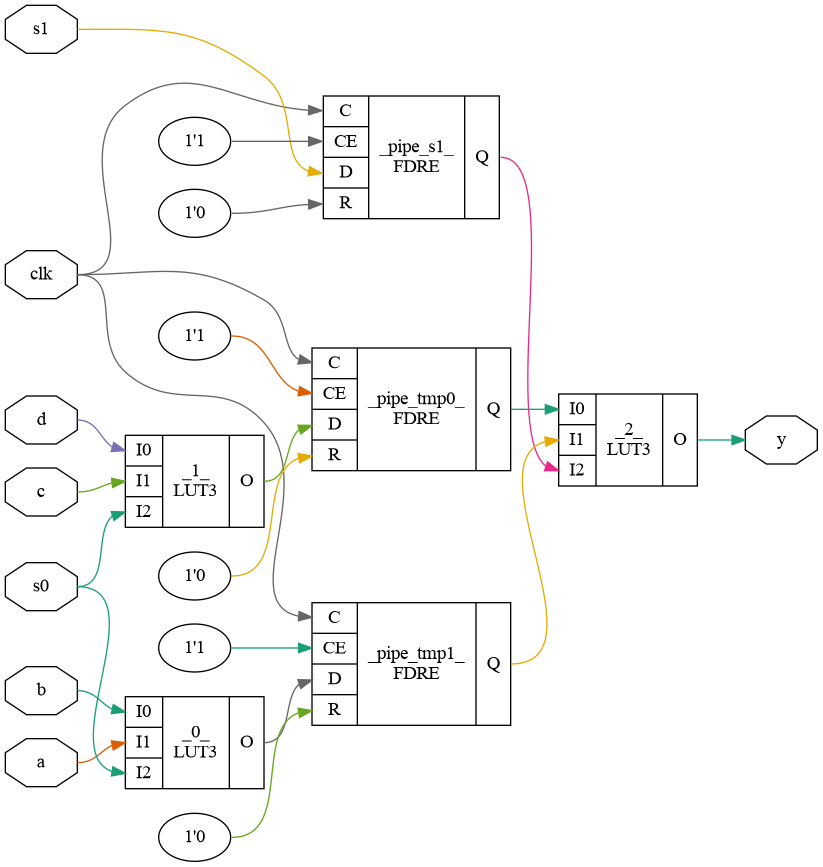
\includegraphics[width=\textwidth]{img/mux_4_1.png}
        \caption{Three 3-LUT, three FF topology.}\label{fig:retiming:a}
        \Description[]{}
    \end{subfigure}
    \begin{subfigure}{0.33\textwidth}
        \centering
        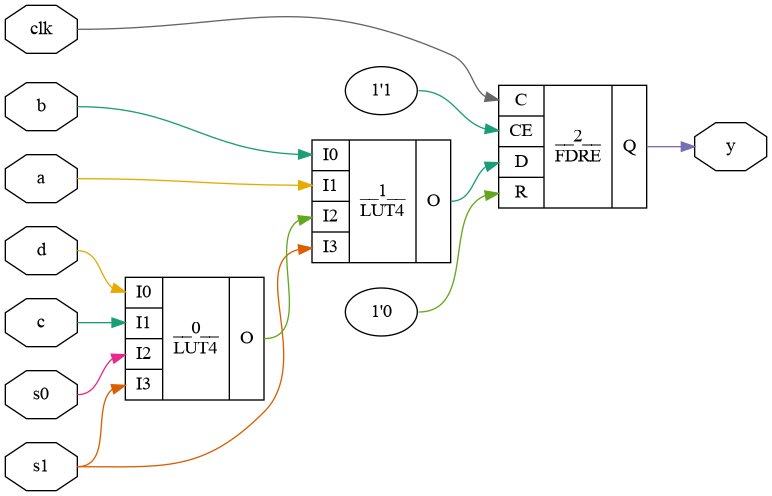
\includegraphics[width=\textwidth]{img/mux_4_1_retime_dsd.png}
        \caption{Two 4-LUT, one FF topology.}\label{fig:retiming:b}
        \Description[]{}
    \end{subfigure}
    \begin{subfigure}{0.33\textwidth}
        \centering
        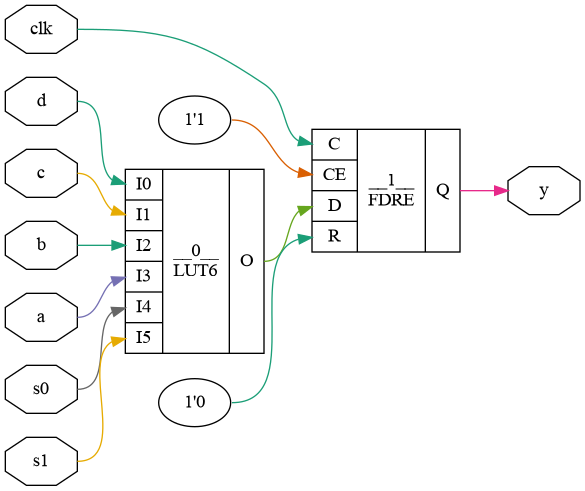
\includegraphics[width=\textwidth]{img/mux_4_1_retime.png}
        \caption{One 6-LUT, one FF topology.}\label{fig:retiming:c}
        \Description[]{}
    \end{subfigure}
    \caption{Three varying topologies for 4:1 MUX with pipeline register. \todo{Placeholder images. Remake by hand.}}\label{fig:retiming}
    \Description[]{}
\end{figure*}

Register retiming, as a purely structural rule, can be implemented with a
simple search and apply pattern. An example for $k=3$ would be written as
follows:

\begin{verbatim}
    (LUT F (REG x0) (REG x1)) <=> (REG (LUT F x0 x1))
\end{verbatim}

Unlike the other rules, this rule is searched for in both directions.
Figure~\ref{fig:retiming} illustrates an example of how register retiming can
compose with LUT rewrite rules to reduce LUT count and register count
simultaneously. In this case, LUTs representing 2:1 multiplexers are push
across register boundaries. Since this logic happens to have a one 6-LUT
packing and two 4-LUT packing, the total LUT count is reduced in conjunction
with register count. Moreover, our cost model can take into account different
weights for flip-flop cells versus LUT cells. E-graph extraction is elaborated
in the next section, but it should be noted that our trials weight LUTs and
registers equally.